\mysubsection{Linda Schey}{DMX-Scheinwerfer}
\label{ssec:DMX}

Für die LED-Scheinwerfer wurden acht \emph{Eurolite LED CLS-18 QCL RGBW} verwendet, die jeweils über einen dreipoligen XLR- Ein- bzw. Ausgang verfügen, so dass sie in Reihe geschaltet über das DMX512 Protokoll mit zwölf Kanälen gesteuert werden können. Ein \emph{Eurolite USB-DMX512-PRO} Interface dient als Schnittstelle zwischen den Lichtern und dem PC. Angesteuert werden die Lichter dann mittels der in \autoref{ssec:entscheidungen} bereits erwähnten Software Freestyler. \autoref{fig:FStoLED} zeigt grob wie die drei Komponenten zusammenhängen. Es wird hier den Pfeilen der Abbildung entsprechend nur in eine Richtung kommuniziert, da das Verhalten der Scheinwerfer ausschließlich durch die Applikation gesteuert wird und keine rückläufige Kommunikation nötig ist.
\begin{figure}[htbp]
	\centering
		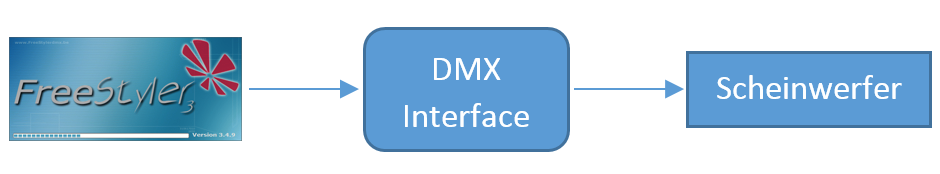
\includegraphics[width=0.90\textwidth]{images/FStoDMXInterfaceToLEDs.PNG}
	\caption{Verknüpfung der Komponenten}
	\label{fig:FStoLED}
\end{figure}
Jeder Scheinwerfer besteht aus 18 LEDs die in drei Reihen mit jeweils sechs LEDs angeordnet sind. Zwei Zeilen, also sechs LEDs, werden in der Applikation jeweils als ein Segment verwendet und kann mit vier Farbkanälen separat angesteuert werden. Insgesamt werden 12 Farbkanäle pro Scheinwerfer eingesetzt. Innerhalb der \enquote{Blinken Tiles} Anwendung gibt es zwei Klassen, die hauptverantwortlich für die Lichtsteuerung sind. \emph{Spot.cs} und \emph{LightController.cs}. \emph{Spot.cs} repräsentiert in der Anwendung einen LED-Scheinwerfer. Diese Klasse verwaltet die Farbwerte für jeden einzelnen Spot und dessen Segmente. In der Klasse \emph{LightController.cs} werden die Farbwerte für alle acht Scheinwerfer in einem Array gespeichert. Dieses Array wird mit den Farbwerten der einzelnen Scheinwerfer befüllt. Die Farbwerte der Scheinwerfer, werden regelmäßig pro Frame aktualisiert. Dabei wird überprüft welcher der Scheinwerfer gerade aktiv sein muss und anhand einer Zeitreferenz welches Segment des Scheinwerfers aktiviert sein soll. Alle anderen Scheinwerfer und deren Segmente werden aus Schwarz gestellt, also nicht leuchtend. 
Jeder Scheinwerfer besteht aus 18 LEDs die in drei Reihen mit jeweils sechs LEDs angeordnet sind. Zwei Zeilen, also sechs LEDs, werden in der Applikation jeweils als ein Segment verwendet und  kann mit vier Farbkanälen separat angesteuert werden. Insgesamt werden also 12 Farbkanäle pro Scheinwerfer eingesetzt. Innerhalb der \enquote{Blinken Tiles} Anwendung gibt es zwei Klassen, die hauptverantwortlich für die Lichtsteuerung sind. \emph{Spot.cs} und \emph{LightController.cs}. \emph{Spot.cs} repräsentiert in der Anwendung einen LED-Scheinwerfer. Die Klasse \emph{Spot.cs} verwaltet die Farbwerte für jeden einzelnen Spot und dessen Segmente. Welchen Farbwerte eingetragen werden wird aus einer Konfigurationsdatei ausgelesen.. In der Klasse \emph{LightController.cs} werden die Farbwerte für alle acht Scheinwerfer in einem Array gespeichert. Die Farbwerte der Scheinwerfer, werden regelmäßig pro Frame aktualisiert. Dabei wird überprüft welcher der Scheinwerfer gerade aktiv sein muss und anhand einer Zeitreferenz welches Segment des Scheinwerfers aktiviert sein soll (\emph{UpdateFaderValues()}. Alle anderen Scheinwerfer und deren Segmente werden auf Schwarz gestellt, nicht leuchtend. 
Um die Scheinwerfer aus der Anwendung \enquote{Blinken Tiles} heraus zu steuern wird ein Zwischenschritt über die Software Freesyler gemacht, da diese Software die Ansteuerung der einzelnen Segmente eines jeden Scheinwerfers sehr komfortabel gestaltet. Um aus \enquote{BlinkenTiles} mit Freestyler zu kommunizieren wurde eine DLL (\emph{LetThereBeLight.dll}) erstellt, die per \emph{FindWindow()} und \emph{SendMessage()} mit zwischen \enquote{Blinken Tiles} und Freestyler vermittelt.


